\documentclass{article}
\usepackage{graphicx} % new way of doing eps files
\usepackage{listings} % nice code layout
\usepackage[usenames]{color} % color
\usepackage{url}
\usepackage{hyperref}
\definecolor{listinggray}{gray}{0.9}
\definecolor{graphgray}{gray}{0.7}
\definecolor{ans}{rgb}{1,0,0}
\definecolor{blue}{rgb}{0,0,1}
% \Verilog{title}{label}{file}
\newcommand{\Verilog}[3]{
  \lstset{language=Verilog}
  \lstset{backgroundcolor=\color{listinggray},rulecolor=\color{blue}}
  \lstset{linewidth=\textwidth}
  \lstset{commentstyle=\textit, stringstyle=\upshape,showspaces=false}
  \lstset{frame=tb}
  \lstinputlisting[caption={#1},label={#2}]{#3}
}


\author{Cameron Anderson}
\title{Project Report: 3D Project}



\begin{document}
\maketitle



\section{Introduction}
The goal of this project is to use the ADXL362 3-axis accelerometer on the Nexys 4 DDR to map a three dimensional environment by moving the board through space. For example, the board could be used to approximately measure three different size boxes. To map the 3D environment, MATLAB would need to be used by taking UART values from the Nexys 4 DDR as it is moved and plotting the mapped values. This and other projects can be seen at the link below.

\begin{center}
\href{https://github.com/camerona254/SoftcoreSoCFPGA.git}{My Softcore SoC FPGA Github Repository}
\end{center}

\section{Experimental Plan}
\subsection{Microblaze Processor}
\begin{figure} 
\begin{center}
	\caption{Microblaze MCS and MMIO Controller}\label{fig:cpu}
	\includegraphics[width=0.9\textwidth]{cpu.jpg}
\end{center}
\end{figure}
The first step of the plan is to implement the Microblaze processor in Vivado Design Suite because the processor will be used to ultimately control the required peripherals for the project. The instantiation of the processor is done from the Project Manager window in Vivado Design Suite when IP Catalog is selected. From the IP Catalog Window, Embedded Processing > Processor > Microblaze MCS are selected. Once the core configuration is complete, the cpu\_unit requires a wrapper to interface with the microprocessor. In this case, the mcs\_top\_vanilla.sv file that Chu provides houses the instantiated microprocessor. 
\subsection{Drivers and Modules}
The second part of the plan is to identify and instantiate the necessary modules for the project. The ADXL362 accelerometer operates as a slave module on an SPI bus. To use the accelerometer, an SPI bus module is needed as is a wrapper for the bus that is used to control the bus and slot it into the MMIO unit in slot 9. Additionally, the data from the accelerometer must be passed to MATLAB via UART protocol. To make a UART bus, Chu provides a UART unit that houses modules for baud rate generation, a receive state machine, a transmit state machine, a fifo rx state machine, and a fifo tx state machine. Chu also provides the wrapper for slotting the UART bus within the MMIO unit in slot 1, as seen in Figure~\ref{fig:cpu} on page~\pageref{fig:cpu}. The MMIO unit is housed in the processor block and has universal slots for peripheral units. Chu provides this module as well for the microprocessor. It is worth noting that had Chu not provided these modules, not all of them would be need. For example, only the UART tx functionality is of interest since this project reads from the SPI bus. 
\subsection{Software Development}
Part 3 of the plan is to create the hardware specs that are the foundation for the software development in Xilinx Software Development Kit. The .hdf file is generated by selecting file, export, and export hardware in Vivado Design Suite. Once the .hdf file is generated, the hardware specs are created by selecting File, New, Other, and Hardware Platform Specifications and then uploading the .hdf file. Part 4 of the experimental plan is to incorporate the hardware specs into a board support package that will contain drivers and start-up routines. This is done in Xilinx SDK by selecting File, New, Other, and Board Support Package. Once the target hardware has been selected and a standalone OS is chosen, the BSP can be generated. The BSP must be generated after the Hardware Platform Project. The fifth part of the project plan is to create a software application. In Xilinx SDK, select File, New, and Application Project. From the menu, a C++ project can be created. Part 6 of the project is to write the necessary software to implement our design. The C++ code needs to initialize the SPI and UART buses, then it needs to continuously read from SPI and write to UART. Lastly, MATLAB needs to take the UART values and plot the corresponding 3D space. 

\section{Analysis}
\subsection{ADXL362 Accelerometer and SPI bus}
\begin{figure}
\begin{center}
\caption{Timing diagram for the ADXL362 SPI Bus}\label{fig:AccelTiming}
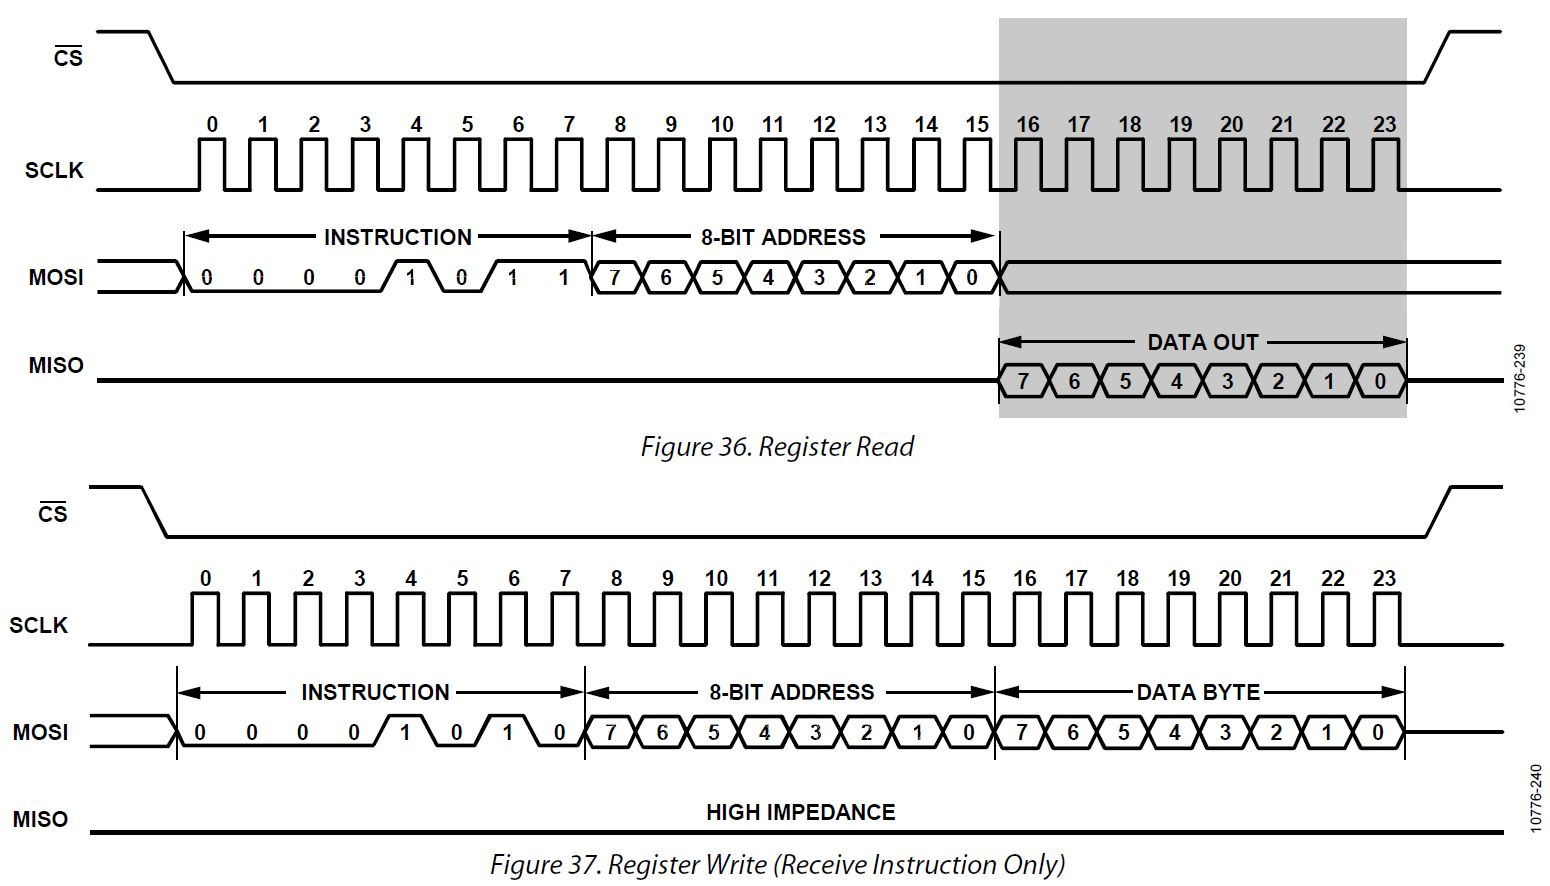
\includegraphics[width=0.9\textwidth]{Timing.jpg}
\end{center}
\end{figure}
To interact with the accelerometer, the SPI bus must be modeled to correctly interface with the device. For example, the slave select signal is an active low signal. Without that knowledge, the accelerometer would not be able to communicate with the processor. The ADXL362 Datasheet is easy to find via a Google search. This first thing that is important to note is the accelerometer's command structure. The datasheet, as seen in Figure~\ref{fig:AccelTiming} on page~\pageref{fig:AccelTiming}, shows the command structure as follows: </CS down> <command byte (0x0A or 0x0B)> <address byte> <data byte> <additional data bytes for multi-byte> … </CS up>. First the chip select is pulled down by the processor. Then a command byte (either read or write) is sent to the accelerometer followed by an address byte. Depending on whether a read or write was sent, a data byte is sent to or from the accelerometer in the following clock cycles. After that depending on how the accelerometer was initialized, either an additional bytes are sent or the chip select can be pulled up. The datasheet also contains information about the clock phase and polarity that the SPI bus should operate on, both of which are 0 in this case. The clock phase and polarity are accounted for in the state machine for the SPI bus and by the function set\_mode in the SPI core C++ header file.
  
\subsection{UART}
UART setup requires that the baud rate be set to match the baud rate of the other component, in this case the PC running MATLAB. This is handled in the function set\_baud\_rate that can be found in the C++ header file for the UART core. It should also be known that the tx register must not be loaded until the whole contents of the register have been sent. This can be done by using the function tx\_empty that is also found in the C++ header file for the UART core.

\subsection{Software}
After recognizing the specific needs of both the SPI and UART buses, the software can be written to read the x, y, and z values from the SPI bus and to write them to the UART bus. First the UART bus is initialized by setting the baud rate at 9600 in the main file and on the PC. Then the SPI is initialized by the set\_mode and set\_frequency functions. The assert\_ss function is then used to assert the chip select after which rd\_data is used to send commands to read each specific directional register and store the values. Once the SPI bus is deasserted with the deassert\_ss function, the x, y, and z register values are sent via six iterations of the rx\_byte function. The first, third, and fifth bytes are the x, y, and z, ascii codes and the second, fourth, and sixth are the corresponding values of the accelerometer measurements for those axes. The rx\_byte function has to be looped to avoid being overwritten. This is done by a while loop and the function rx\_fifo\_empty.

\section{Conclusion}
This hardware portion of this project was implemented successfully after debugging. Synthesis, Implementation, and Bitstream Generation have run with no errors or warnings. However, despite spending a great deal of time debugging, this project was not successful is reading the accelerometer or transferring the data to the UART bus which supports the idea that the software component was not complete.  

\end{document} 